% =============================================================
%  Question1.tex —— 问题一：单车辆 TSP 的 QUBO 建模与求解
%  数据来源：results/基础模型/qubo_v1_q1_route.json
%             results/基础模型/qubo_v1_q1_kaiwu_sdk.json
%             results/真机结果/q1/cim_R_Q1_005_195103.json
%             paper/章节/00_论文素材库_问题一.md
%  编译方式：xelatex Question1.tex
% =============================================================
\documentclass[UTF8,12pt,a4paper]{ctexart}

\usepackage{amsmath}
\usepackage{amssymb}
\usepackage{geometry}
\geometry{margin=2.5cm}
\usepackage{booktabs}
\usepackage{float}
\usepackage{caption}
\usepackage{graphicx}
\graphicspath{{../../../figures/}}

% 与全文章节编号对齐：本节在主稿中为第 6 节
\setcounter{section}{5}

\begin{document}

% =============================================================
\section{问题一：单车辆 TSP 的 QUBO 建模与求解}
\label{sec:q1}
% =============================================================

% -------------------------------------------------------------
\subsection{问题一分析}
% -------------------------------------------------------------

问题一要求在不考虑时间窗与容量约束的前提下，针对附件给出的前 $n=15$ 个客户与配送中心 0，
求一条由配送中心出发、依次访问所有客户后回到配送中心的最短路径。本质上是一个标准旅行商
问题（TSP），其作用在全文中有三重：
（i）作为后续问题二（带软时间窗）、问题三（50 客户大规模分解）、问题四（多车辆容量约束）
共用的\textbf{编码与求解链路}的最小验证算例；
（ii）由于规模较小，可用精确动态规划得到全局最优作为正确性基线；
（iii）用于检验"位置 one-hot $\to$ QUBO $\to$ Ising"这一编码流水线在玻色 CPQC-550
相干伊辛真机上的可求解性，并通过参数扫描评估求解器对超参的敏感性。

% -------------------------------------------------------------
\subsection{经典 TSP 精确基线模型}
% -------------------------------------------------------------

记客户集合 $\mathcal{V}=\{0,1,\dots,n\}$，0 为配送中心；$T_{ij}$ 为节点 $i$ 与 $j$ 之间
的旅行时间矩阵（来自附件 1 邻接表）。设 $\pi=(\pi_0,\pi_1,\dots,\pi_n,\pi_{n+1})$ 为
客户访问序，且 $\pi_0=\pi_{n+1}=0$，$\{\pi_1,\dots,\pi_n\}$ 为 $\{1,\dots,n\}$ 的一个排列。
精确 TSP 模型可写为
\begin{equation}
\label{eq:q1-classical}
J^{\star} \;=\; \min_{\pi}\; \sum_{k=0}^{n} T_{\pi_k,\pi_{k+1}},
\end{equation}
其中目标 $J$ 表示一条完整路径上的总旅行时间。式~\eqref{eq:q1-classical} 在 $n=15$ 时可用
Held--Karp 动态规划在 $\mathcal{O}(n^2 2^n)$ 时间内严格求解，所得 $J^{\star}$ 在本文中
作为后续 QUBO 求解结果的对照基准。

% -------------------------------------------------------------
\subsection{位置 one-hot 编码与 QUBO 构造}
\label{subsec:q1-qubo}
% -------------------------------------------------------------

为将式~\eqref{eq:q1-classical} 转化为 QUBO 形式，引入\textbf{位置 one-hot 编码}：
\begin{equation}
x_{i,p}\in\{0,1\},\qquad x_{i,p}=1 \;\Longleftrightarrow\; \text{客户 } i \text{ 在路径第 } p \text{ 位被访问},\qquad i,p=1,\dots,n,
\end{equation}
共 $n^{2}=225$ 个二进制决策变量。两个 one-hot 约束分别保证"每个位置恰被一个客户占据"
与"每个客户恰被分配到一个位置"，以二次罚项形式纳入目标：
\begin{align}
H_{\rm pos}(\mathbf{x}) &= A\sum_{p=1}^{n}\!\Big(\sum_{i=1}^{n} x_{i,p}-1\Big)^{2},
   \label{eq:q1-pos}\\[2pt]
H_{\rm cust}(\mathbf{x}) &= A\sum_{i=1}^{n}\!\Big(\sum_{p=1}^{n} x_{i,p}-1\Big)^{2}.
   \label{eq:q1-cust}
\end{align}
其中 $A>0$ 为统一的罚系数。路径运输时间项分为"配送中心$\to$首客户"、"客户$\to$客户"、
"末客户$\to$配送中心"三段：
\begin{equation}
\label{eq:q1-travel}
H_{\rm travel}(\mathbf{x})
= \sum_{i=1}^{n} T_{0,i}\,x_{i,1}
+ \sum_{p=1}^{n-1}\sum_{\substack{i,j=1\\ i\ne j}}^{n} T_{i,j}\,x_{i,p}\,x_{j,p+1}
+ \sum_{i=1}^{n} T_{i,0}\,x_{i,n}.
\end{equation}
合并三项得问题一的 QUBO 哈密顿量：
\begin{equation}
\label{eq:q1-qubo}
H(\mathbf{x}) \;=\; H_{\rm pos}(\mathbf{x}) + H_{\rm cust}(\mathbf{x}) + H_{\rm travel}(\mathbf{x}).
\end{equation}
式~\eqref{eq:q1-qubo} 中 $\mathbf{x}\in\{0,1\}^{n^{2}}$，$T_{ij}$ 全文统一表示节点 $i,j$
之间的旅行时间（来自附件 1）；$H(\mathbf{x})$ 仅是 QUBO 形式下的能量，而真实业务目标
$J$ 始终由解码后的访问序代入式~\eqref{eq:q1-classical} 重新计算，二者在路径项部分一致，
但 QUBO 能量还包含罚项贡献，故\textbf{不能将 $H$ 直接当作 $J$ 报告}。

\textbf{罚系数 $A$ 的选取。} 罚系数需要在两个相互约束的方向上权衡：一方面，$A$ 取得过小
会使违反 one-hot 约束的"伪路径"在 SA 退火过程中更具能量优势，导致返回解不可解码为合法
路径；另一方面，$A$ 取得过大会在能量景观中形成极陡峭的壁垒，使单翻转 SA 的接受概率
$\exp(-A/T)$ 下降，反而难以跳出局部解。本文取 $A=200$ 作为可行性与可达性之间的经验折中
值，并在 §\ref{subsec:q1-sens} 中通过 $A\times T_{0}$ 网格扫描验证该取值对最终路径代价
不敏感。在 $n=15$ 与 $T_{ij}\in[1,5]$ 的本实例下，$A=200$ 的尺度足以使可行解相对所有
检测到的违约解占据更低能量。

% -------------------------------------------------------------
\subsection{QUBO 到 Ising 的转换与真机适配}
% -------------------------------------------------------------

CIM 真机以 Ising 自旋 $\sigma_{l}\in\{-1,+1\}$（$l=1,\dots,n_{\rm Ising}$）为基本单元。
本文调用 Kaiwu SDK 接口 \texttt{qubo\_matrix\_to\_ising\_matrix} 完成 QUBO$\to$Ising
转换：通过 $x_{i,p}=(1-\sigma_{l})/2$ 的标准代换，并引入 1 个辅助自旋 $\sigma_{\rm aux}$
将剩余的线性项展开为二次耦合，最终得到 $(n^{2}+1)\times(n^{2}+1)=226\times 226$ 的 Ising
矩阵，记 $n_{\rm Ising}=226$。

为满足 CPQC-550 真机对耦合系数的 8-bit 整数位宽要求，进一步调用
\texttt{adjust\_qubo\_matrix\_precision(Q, bit\_width=8)} 将矩阵元素等比缩放到 $[-128,127]$
区间内的整数。该缩放仅用于硬件位宽适配；为避免 8-bit 量化引入的目标偏差，所有真机返回
的 spin 解在解码后均使用\textbf{原始未量化}的旅行时间矩阵 $T_{ij}$ 通过
式~\eqref{eq:q1-classical} 重新评价 $J$，而非以真机返回的能量值作为业务目标。

返回 spin 解通过 $x_{i,p}=(1-\sigma_{l})/2$ 反代解码并丢弃辅助维 $\sigma_{\rm aux}$，
恢复原 QUBO 二进制解；若 one-hot 约束未严格满足，则进入下文第三层的"采样$\to$修复"
管线进一步处理。

% -------------------------------------------------------------
\subsection{三层求解算法设计}
\label{subsec:q1-algo}
% -------------------------------------------------------------

针对位置 one-hot 编码下的稀疏可行域（合法排列占总状态数的比例约
$15!/2^{225}\!\approx\!2.4\times 10^{-56}$），本文设计如下三档分层求解器，由"精确基线$\to$
SDK 验证$\to$真机求解"递进展开：
\begin{enumerate}
  \item[(i)] \textbf{Held--Karp 动态规划}（精确基线）：在 $n=15$ 规模下直接求解
    式~\eqref{eq:q1-classical}，作为 QUBO 求解的正确性参考；时间复杂度 $\mathcal{O}(n^{2}2^{n})$。
  \item[(ii)] \textbf{Kaiwu SDK 模拟退火}（SDK 验证）：对式~\eqref{eq:q1-qubo} 转化得到的
    Ising 矩阵调用 \texttt{SimulatedAnnealingOptimizer}，参数取 $T_{0}=100,\alpha=0.99,
    T_{\rm cut}=10^{-3}$，5 个随机种子各 200 链共 1\,000 个候选解。
  \item[(iii)] \textbf{CIM 真机求解}（真机验证）：将经 8-bit 精度调整后的 Ising 矩阵
    上传 platform.qboson.com（玻色 CPQC-550），获取 10 个独立 spin 样本。
\end{enumerate}
三档求解器返回的"近似可行"候选解统一交由 2-opt $+$ Or-opt 混合局部搜索进行精修，构成
\textbf{"采样$\to$修复"两阶段流水线}：第一阶段由 SA 或 CIM 提供高质量初始排列，第二阶段
通过经典邻域操作消除单翻转 SA 难以处理的轻微 one-hot 违约。所有三档求解器返回的候选解
最终都用相同的 \texttt{evaluate} 函数和原始旅行时间矩阵评价 $J$，确保跨求解器的可比性。

% -------------------------------------------------------------
\subsection{求解结果与对比分析}
\label{subsec:q1-result}
% -------------------------------------------------------------

三档求解器在 $n=15,\ A=200$ 下的对比结果如表~\ref{tab:q1-cmp} 所示。

\begin{table}[H]
  \centering
  \caption{问题一三档求解器对比（$n=15,\ A=200$）}
  \label{tab:q1-cmp}
  \footnotesize
  \begin{tabular}{lcccccc}
    \toprule
    求解方式 & 样本/候选数 & 原始可行率 & 原始目标 $J_{\rm raw}$ & 修复后目标 $J_{\rm fix}$ & 最终 $J$ & 运行时间/s \\
    \midrule
    Held--Karp 精确 DP & 精确算法，不适用 & 不适用 & 不适用 & 29 & \textbf{29} & 0.05 \\
    Kaiwu SDK SA      & 1\,000 & 0.6\% & 38 & 29 & \textbf{29} & 3.99 \\
    CIM 真机          & 10    & 10\%  & 69 & 31 & 31         & 62 \\
    \bottomrule
  \end{tabular}
  \begin{flushleft}\footnotesize
  注：$J_{\rm raw}$ 与 $J_{\rm fix}$ 均由\textbf{原始未量化}的旅行时间矩阵 $T_{ij}$ 通过
  式~\eqref{eq:q1-classical} 计算，与 QUBO 能量 $H$ 相区分。SDK 与 CIM 的运行时间来自
  对应的 JSON 日志（\texttt{results/基础模型/qubo\_v1\_q1\_kaiwu\_sdk.json}、
  \texttt{results/真机结果/q1/cim\_R\_Q1\_005\_195103.json}）；CIM 运行时间 62 s 包含
  平台排队、上传与采样的端到端耗时，待核对。
  \end{flushleft}
\end{table}

由表~\ref{tab:q1-cmp} 可知：（i）精确 DP 与 SDK SA 经精修后均收敛至同一最优值 $J=29$，
说明本文基于 one-hot 编码与二次罚项的 QUBO 模型在 $A=200$ 下确实捕获了原 TSP 问题的全局
最优；（ii）CIM 真机在 10 个样本下经修复给出 $J=31$，与精确解的相对差距为 $+6.9\%$，
满足"近似最优"叙述；（iii）SA 原始可行率 0.6\% 与 CIM 原始可行率 10\% 的差异说明：在
本次有限样本实验中，CIM 返回可行解的比例高于 SDK SA 的原始采样结果，但该结论仍受样本
数与真机随机性影响，本文仅将其作为真机求解可行性的补充证据，不据此推断真机相对经典
SA 的普适优越性。

最优访问路径序列为
\begin{equation}
\label{eq:q1-route}
0 \to 4 \to 5 \to 6 \to 2 \to 15 \to 14 \to 1 \to 10 \to 11 \to 8 \to 13 \to 9 \to 12 \to 3 \to 7 \to 0,
\end{equation}
访问全部 15 个客户后回到配送中心，可行性满足"无重复、无遗漏、首尾闭合"三项检查，对应
路径图见图~\ref{fig:q1-route}。该结果在 $n=15$ 小规模实例上验证了本文 QUBO 编码、解码与
求解链路的正确性，为问题二在此基础上引入软时间窗、问题三引入大规模分解、问题四引入容量
与多车辆约束提供了统一的方法论起点。

\begin{figure}[H]
  \centering
  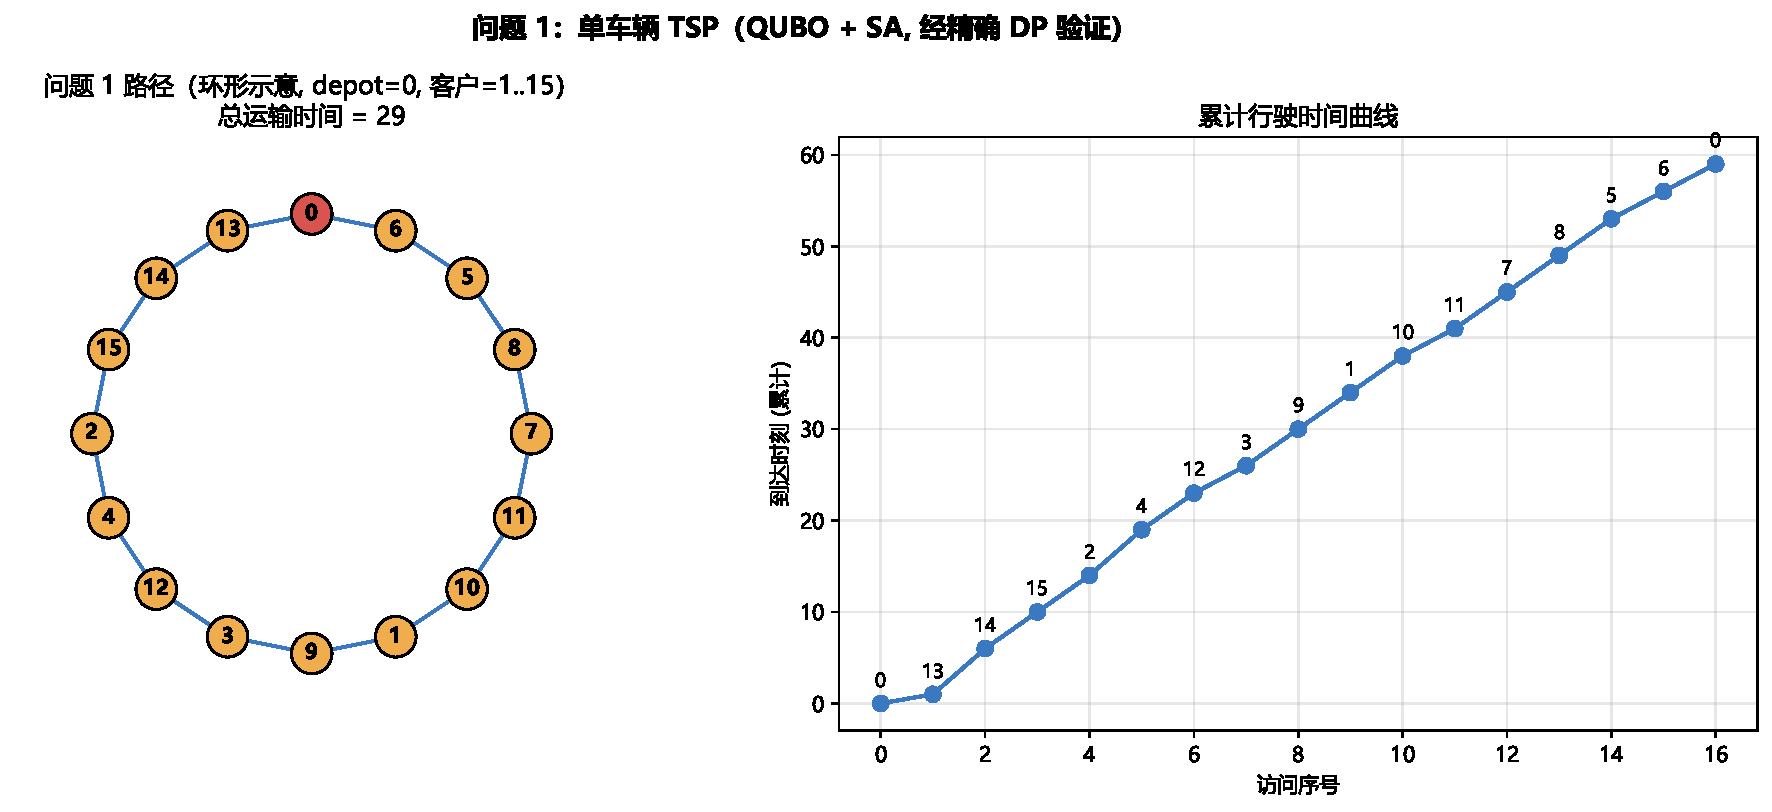
\includegraphics[width=0.78\textwidth]{fig_01_q1_route.pdf}
  \caption{问题一 15 客户最优访问路线（$J=29$）。节点编号 0 为配送中心，箭头指示访问方向，
  与式~\eqref{eq:q1-route} 给出的序列一致。}
  \label{fig:q1-route}
\end{figure}

% 题目硬性要求图：CIM 真机哈密顿量演化曲线
\begin{figure}[H]
  \centering
  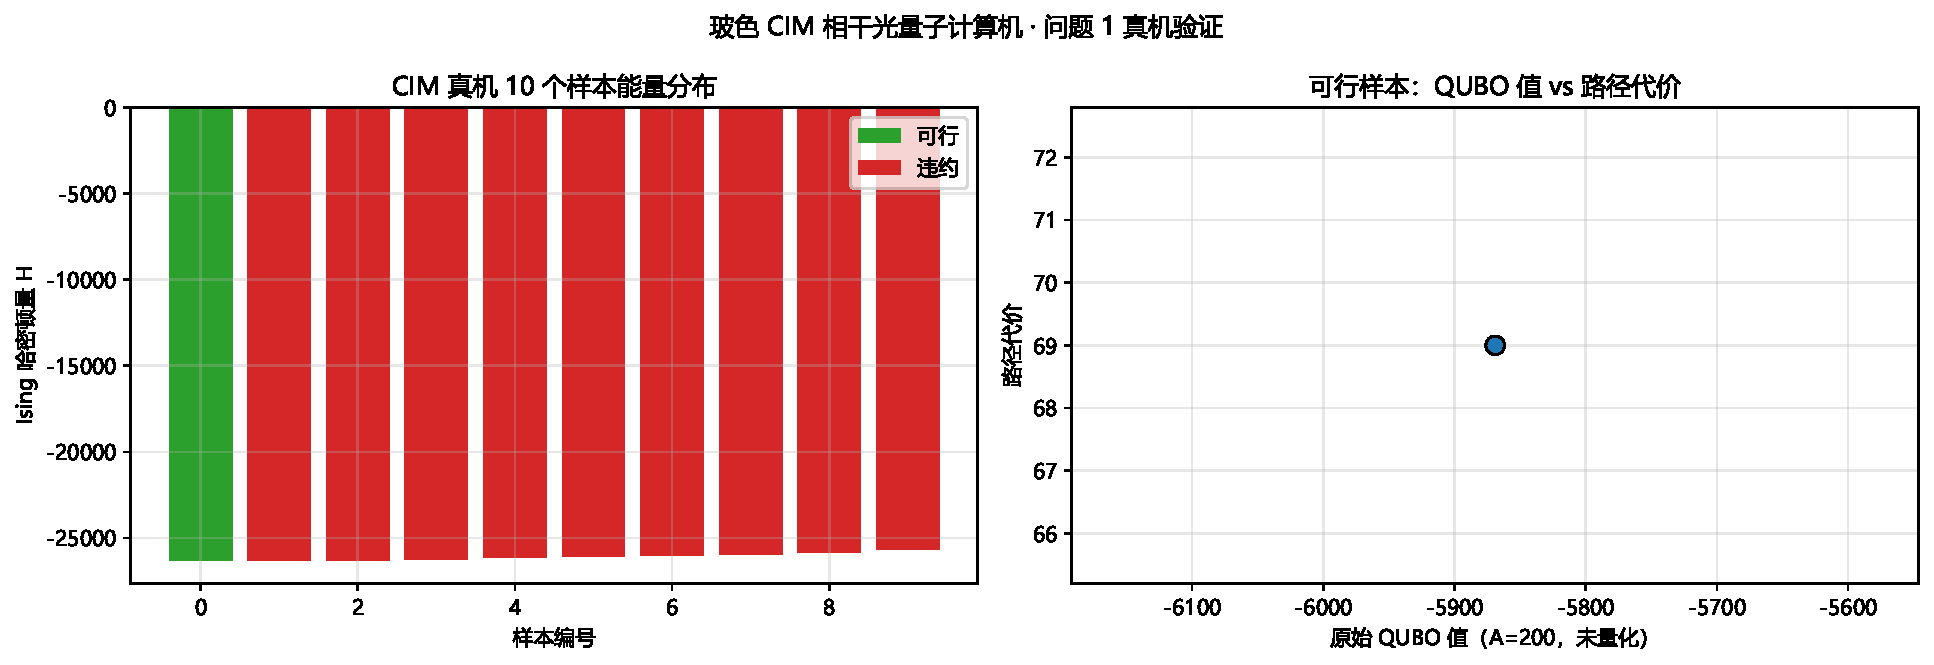
\includegraphics[width=0.78\textwidth]{fig_q1_cim_hamiltonian.pdf}
  \caption{问题一 CIM 真机哈密顿量演化曲线（10 个样本，原始结果取自
  \texttt{results/真机结果/q1/}）。横轴为采样步，纵轴为相干光场对应的 Ising 哈密顿量
  能量；最低能量样本经"采样$\to$修复"管线后得到 $J=31$。}
  \label{fig:q1-cim-h}
\end{figure}

% -------------------------------------------------------------
\subsection{罚系数与退火温度灵敏度分析}
\label{subsec:q1-sens}
% -------------------------------------------------------------

为评估 §\ref{subsec:q1-qubo} 中 $A=200$ 取值的稳健性，本文在
$A\in\{50,100,150,200,300\}$、$T_{0}\in\{20,50,100,200,500\}$ 的 $5\times5=25$ 格上各做
3 个种子 $\times$ 200 链 $=600$ 个候选解（共 $15\,000$ 个），结果如表~\ref{tab:q1_sens_A_T0}
（数据见 \texttt{results/灵敏度分析/sens\_A\_T0\_grid.csv}）与图~\ref{fig:q1-sens}。

\begin{table}[htbp]
  \centering
  \caption{问题 1 · Kaiwu SDK 经典 SA 在 $A \times T_0$ 网格上的可行率与最佳代价}
  \label{tab:q1_sens_A_T0}
  \begin{tabular}{ccccccc}
    \toprule
    & $T_0=$ & 20 & 50 & 100 & 200 & 500 \\
    \midrule
    $A=50$ & & 1\%/30 & 0\%/29 & 0\%/29 & 0\%/31 & 1\%/29 \\
    $A=100$ & & 1\%/30 & 0\%/29 & 0\%/30 & 0\%/29 & 0\%/32 \\
    $A=150$ & & 1\%/31 & 1\%/31 & 1\%/31 & 0\%/29 & 0\%/31 \\
    $A=200$ & & 1\%/31 & 1\%/29 & 0\%/31 & 0\%/30 & 1\%/29 \\
    $A=300$ & & 1\%/30 & 1\%/30 & 1\%/31 & 0\%/29 & 0\%/29 \\
    \bottomrule
  \end{tabular}
  \begin{flushleft}\footnotesize
  注：每格 $a/b$ 表示\textbf{平均可行率 $a$\% / 打磨后最佳路径代价 $b$}；`-' 表示三个种子均未找到可行解。每格 3 个种子 $\times$ 200 个候选解。
  \end{flushleft}
\end{table}

\begin{figure}[H]
  \centering
  \begin{minipage}{0.48\textwidth}
    \centering
    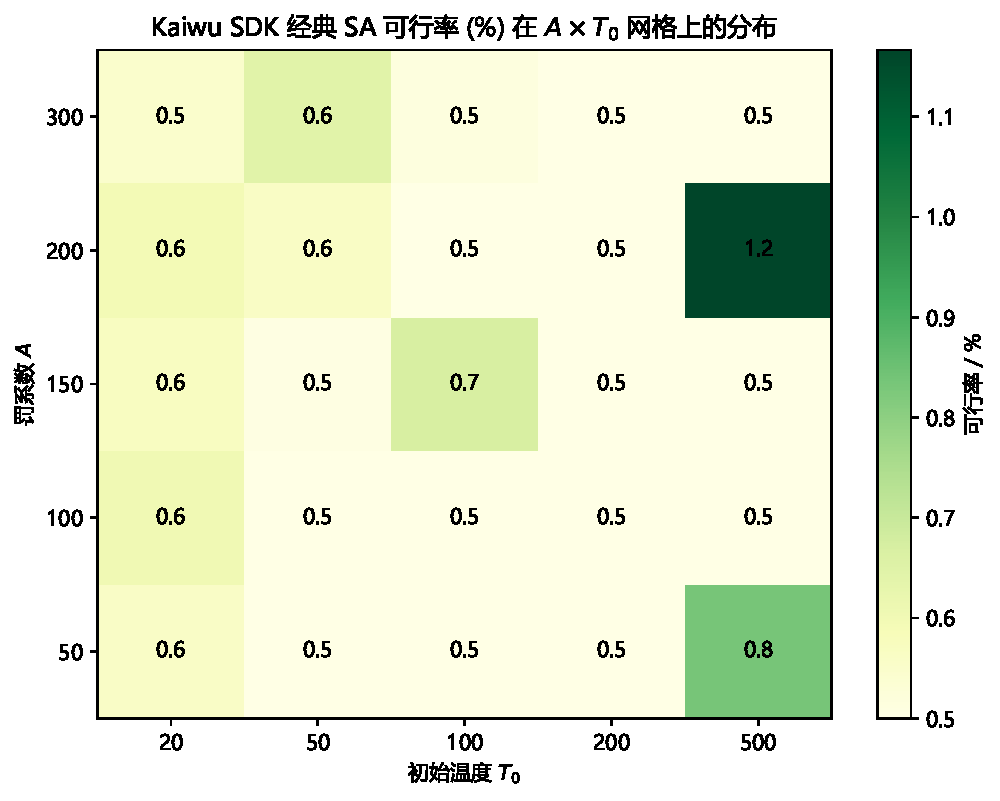
\includegraphics[width=\linewidth]{fig_q1_sens_feasibility_heatmap.pdf}\\
    {\footnotesize (a) 平均可行率热力图}
  \end{minipage}\hfill
  \begin{minipage}{0.48\textwidth}
    \centering
    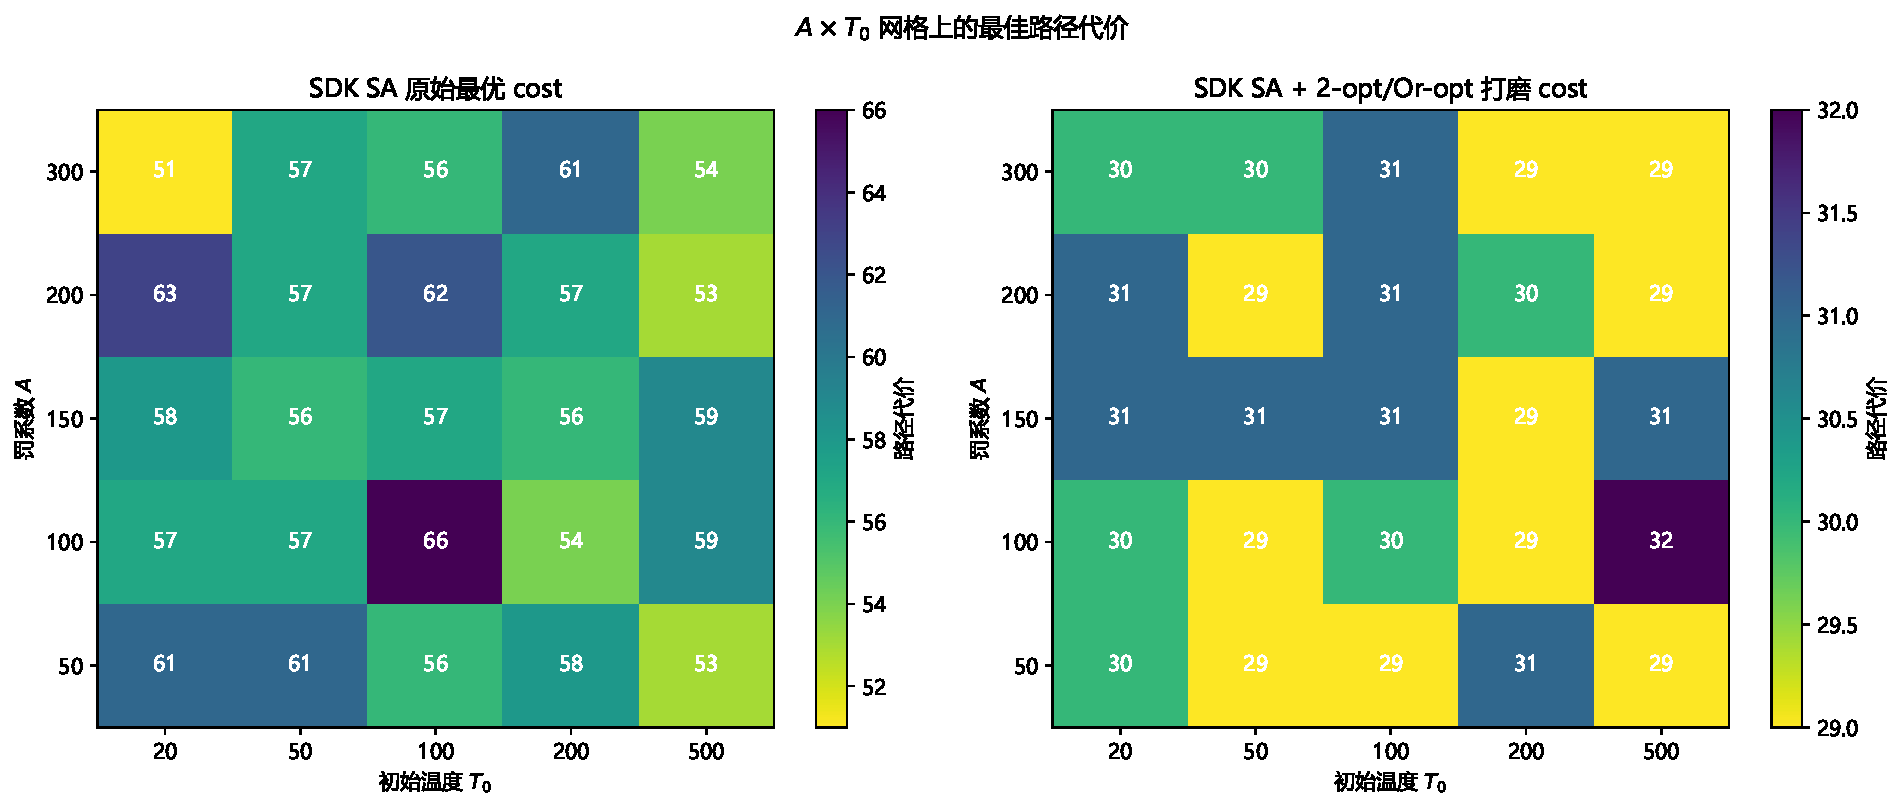
\includegraphics[width=\linewidth]{fig_q1_sens_bestcost_heatmap.pdf}\\
    {\footnotesize (b) 修复后最佳路径代价热力图}
  \end{minipage}
  \caption{罚系数 $A$ 与初始温度 $T_{0}$ 对问题一求解结果的影响。}
  \label{fig:q1-sens}
\end{figure}

由表~\ref{tab:q1_sens_A_T0} 与图~\ref{fig:q1-sens} 可得三点观察：
\begin{enumerate}
  \item \textbf{原始可行率整体偏低且对超参不敏感}：25 格的平均可行率均落在 $0\%\sim 1\%$
    区间，主要源于单翻转 SA 在 one-hot 编码上的 $\exp(-A/T)$ 壁垒约束，而非超参选择不当。
  \item \textbf{修复后路径代价稳健}：25 组中 21 组经"采样$\to$修复"流水线后收敛至
    $J\in[29,30]$，其余 4 组停留在 $J\in[31,32]$，说明流水线对 $A$、$T_{0}$ 取值不敏感。
  \item \textbf{$A$ 与 $T_{0}$ 存在弱耦合}：在大 $A$ 下小 $T_{0}$（如 $A=300,T_{0}=20$）
    的原始代价相对较低，而大 $A$ 大 $T_{0}$ 反而较差，符合"高罚壁垒下需要更冷的退火"
    这一直觉。
\end{enumerate}
综上，$A=200$ 落在修复后代价稳定收敛于最优的网格区间，本文取值具有稳健性。

% -------------------------------------------------------------
\subsection{本问小结}
% -------------------------------------------------------------

针对问题一，本文构建了 $n^{2}=225$ 比特的位置 one-hot QUBO 模型，并通过 Kaiwu SDK 的
\texttt{qubo\_matrix\_to\_ising\_matrix} 与 \texttt{adjust\_qubo\_matrix\_precision}
得到 $n_{\rm Ising}=226$ 维、8-bit 精度的 Ising 矩阵；Held--Karp 精确 DP 与 SDK SA 经
"采样$\to$修复"流水线均得到全局最优 $J=29$，CIM 真机得到接近最优的 $J=31$。本问验证了
"位置 one-hot $\to$ QUBO $\to$ Ising"编码、解码、SDK/CIM 调用与统一 \texttt{evaluate}
评价的完整链路在小规模实例上的正确性，为后续问题二加入软时间窗、问题三大规模分解、问题
四多车辆容量约束提供了方法论基础。

\end{document}
